%% vim: set tw=0 wm=0 wrap linebreak:
\title{Sample Return Challenge Proposal}
\author{
        Russel Howe\\
            \and
        Jascha Little\\
		    \and
	    Zac Lizer\\
}
\date{\today}

\documentclass[12pt]{article}
\usepackage{graphicx}
\usepackage{grffile}
\usepackage{hyperref}
\graphicspath{{./assets/}}
\begin{document}
\maketitle

\begin{abstract}
Our robot uses a primarily visual perception and navigation system, with multiple sets of cameras performing the tasks of navigation and mapping, obstacle avoidance, object detection, and manipulation control. A custom chassis has been designed to minimize weight and ease planning by allowing very general motion over varied terrain. A simple three-axis manipulator takes advantage of this flexibility to allow object retrieval and storage in a sectioned carousel.

\end{abstract}

%\subsection{DESCRIPTION of work to be done between now and the competition}
%-Finish object detector\\
%Finish color discrimination, ground plane intersection\\
%-Home platform detector\\
%Implement a system for visually detecting the home platform and placing it in the world. Presumably this is an extension of the object detector.\\
%-Fix navigation brittleness\\
%The current VSLAM implementation is not adequate for tracking the robot over the full length of a path that covers the entire search area. This has motivated the notion of a radial search pattern, with the robot venturing in as straight a line as possible away from the starting platform until a boundary is reached, then returning to the home platform along the next radius in the circle. Something is needed to 'reset' the navigation system upon reaching or nearing the home platform, as well as overriding the 'search' navigation state with the 'home' navigation state.\\
%-State Machine\\
%Top-level control of the robot that manages which objects have been retrieved, time remaining, distance from the home platform, etc.\\
%-Manipulator\\
%Control and scripting of the gripper to execute a descend, grip, lift routine\\
%-Motion Planning\\
%Routing around local obstacles and return to the nominal search path, approaching the detected sample to be retrieved\\
%-Grip Planning\\
%Handoff from the object detector to the manipulator stereo pair to continue tracking the targeted object and to plan the orientation of the gripper during the grasping routine.\\
%-Pause Switch\\
%Implementation of the system-level pause switch and remote control. This will presumably occur in the state machine.\\
%-Search Planning\\
%Design (distance to travel away from home platform, angular separation of out and return spokes) of the searh pattern and implementation at the state machine level.\\
%-Finalize Mechanicals\\
%Swap out pneumatic tires for tweels, remount and wire new carousel motor


\section{Introduction}
This proposal documents our thought process leading up to the prototype design of a robot to compete in the sample return challenge \cite{rules}. We focus on readily available components and technologies with the goal of getting quickly to the testing phase of our design. For the prior year's competition, we fabricated a custom chassis and began software development of its control system. This year's effort builds on this work.

\paragraph{Outline}
The remainder of this article is organized as follows.
Section~\ref{Chassis} describes the locomotion and maneuvering system. Section~\ref{Manipulator} describes our approach to sample acquisition and storage. Section~\ref{Electronics} describes the power management, servo, and compute systems employed. Section~\ref{Perception} discusses our sensing systems. Section~\ref{Software} gives a high-level overview of our software architecture. Section~\ref{Hazardous} discusses hazardous materials compliance. Section~\ref{Comms} describes the external communications of the robot.


%\begin{figure}[htbp]
%\centering
%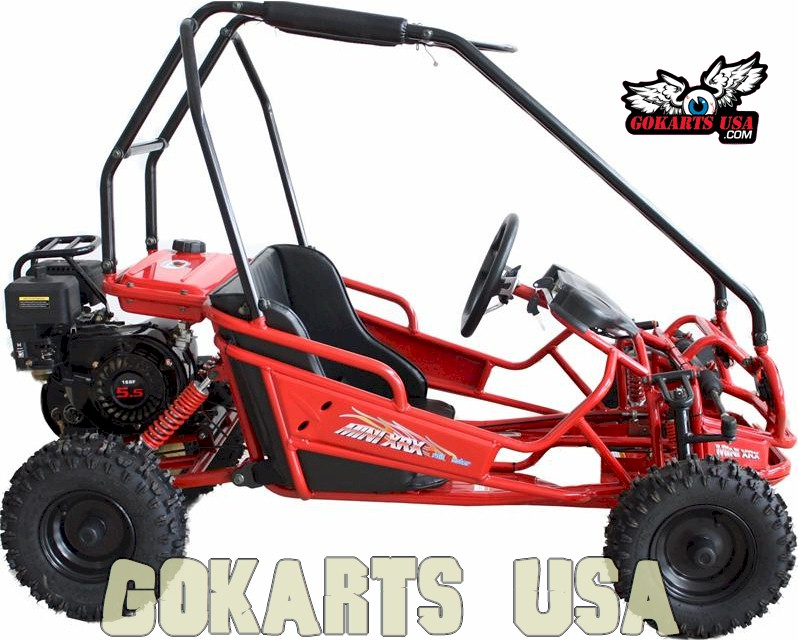
\includegraphics[width=4in]{../assets/TrailMasterMINIXRS.jpg}
%\caption{Labeled Three-Quarters View}
%\label{fig_gokart}
%\end{figure}
%
%\begin{figure}[htbp]
%\centering
%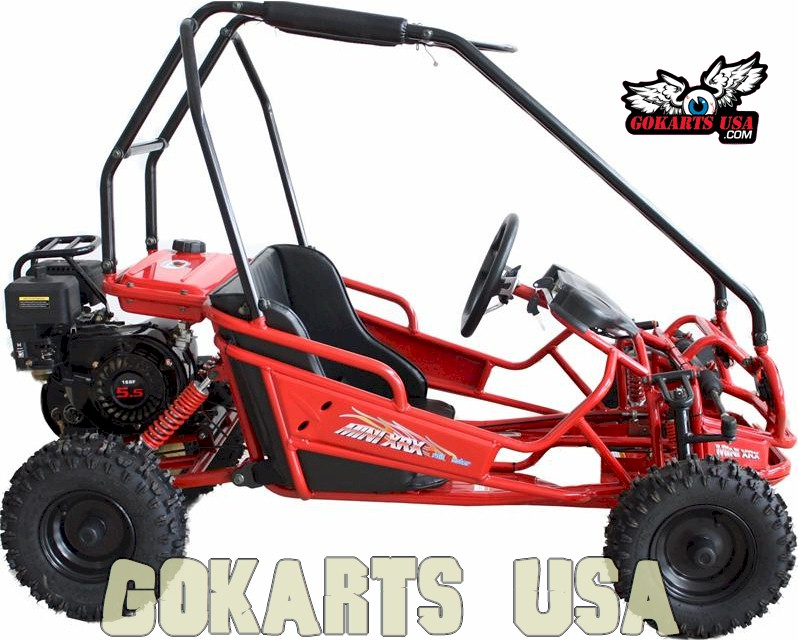
\includegraphics[width=4in]{../assets/TrailMasterMINIXRS.jpg}
%\caption{Wheel Pod}
%\label{fig_gokart}
%\end{figure}
%
%\begin{figure}[htbp]
%\centering
%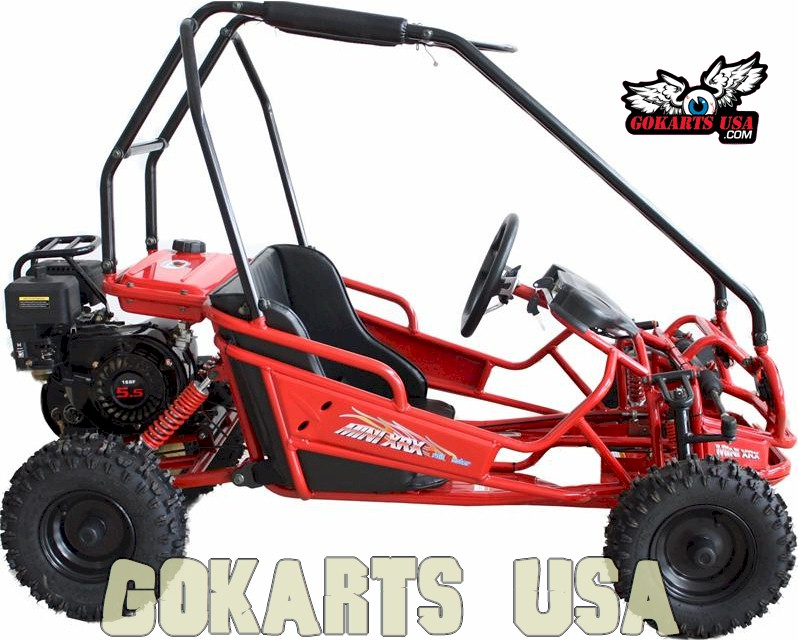
\includegraphics[width=4in]{../assets/TrailMasterMINIXRS.jpg}
%\caption{Manipulator Assembly}
%\label{fig_gokart}
%\end{figure}

\section{Chassis}\label{Chassis}

We fabricated a custom, triangular plan chassis with three independently steerable wheel pods, one on each corner (the side between two wheels defining the front of the robot, with a trailing third). Each wheel pod consists of a wheel and tire driven through a gearbox and chain reduction/transmission by a brushless electric motor. Using three independently steerable wheels allows for in-place rotations of the robot, as well as translation in any direction relative to the manipulator, permitting a simple three-axis manipulator design (up/down, open/close, rotate). Both the drive axis and steering axis for each wheel pod have optical encoders for measuring angle/velocity and aiding the odometry system.

The body itself is a triangular box, providing three distinct mounting layers: under the bottom plate, between the plates, and on the top plate. A sectioned carousel slung under the lower plate is used for sample storage. Indexed by a single motor, its low to the ground position reduces the amount of travel needed in the vertical manipulator axis. Behind the carousel are the lithium ion battery packs, mounted low to keep the center of mass as far down as possible. Between the two triangular decks are the six wheel motor controllers, driving the two motors on each of the three wheel pods. The search and navigation computers are also mounted on this level.

The top plate supports navigation, manipulator, and search cameras, as well as the supports for the manipulator vertical axis. The manipulator cameras peer through a cutout in the lower deck to observe the gripper jaws and the object to be retrieved, as well as the appropriate carousel slot when it's rotated into position. Space is reserved for the specified required payload.

The navigation and search cameras are mounted at the top of a pyramidal frame above the top deck. This provides maximum height above the ground given the volume envelope, expanding the search region

%\begin{figure}[htbp]
%\centering
%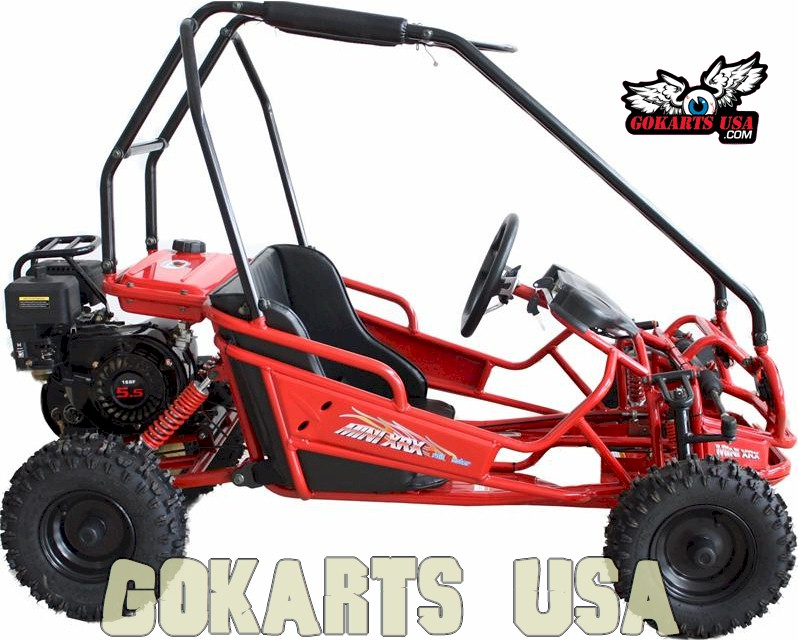
\includegraphics[width=4in]{../assets/TrailMasterMINIXRS.jpg}
%\caption{A possible commercial chassis.}
%\label{fig_gokart}
%\end{figure}


\begin{figure}[htbp]
\centering
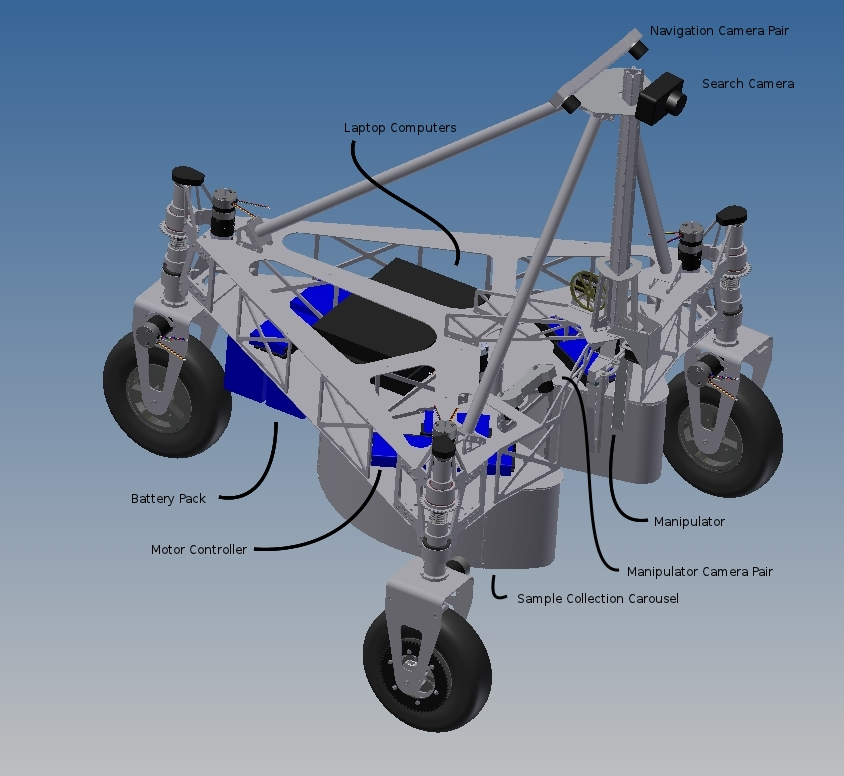
\includegraphics[width=4.5in]{../assets/overalliso.jpg}
\caption{The proposed vehicle chassis.}
\label{fig_bot_chassis}
\end{figure}

\begin{figure}[htbp]
\centering
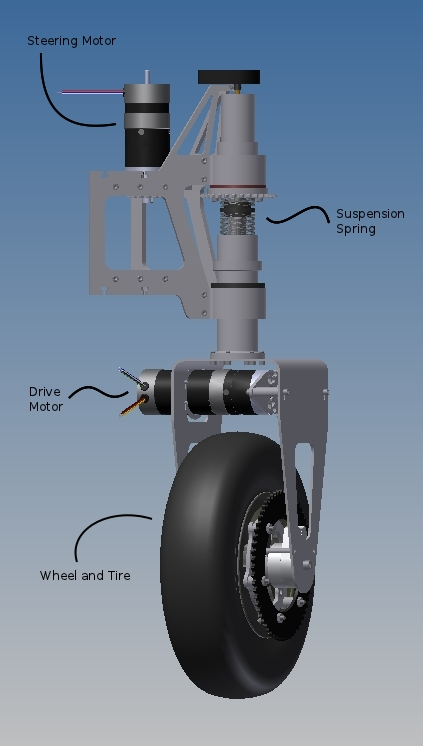
\includegraphics[width=4in]{../assets/wheelmodule.jpg}
\caption{The wheel module.}
\label{fig_bot_wheel}
\end{figure}

\begin{figure}[htbp]
\centering
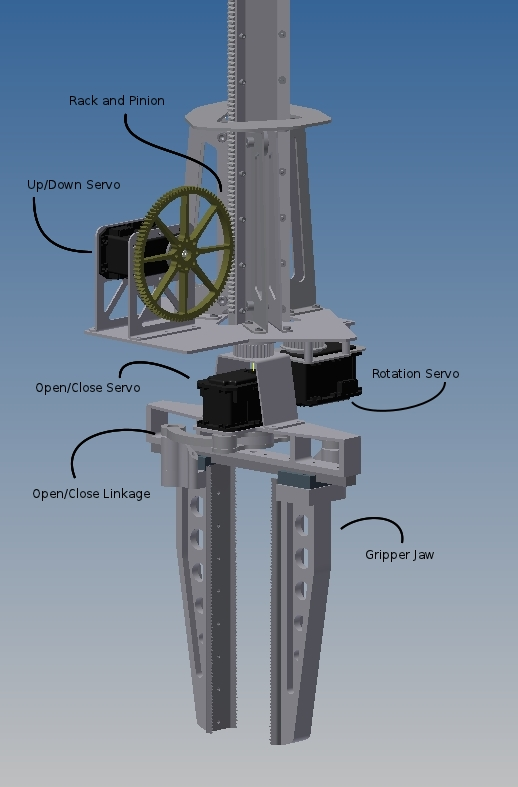
\includegraphics[width=4.5in]{../assets/manipulator.jpg}
\caption{The manipulator.}
\label{fig_bot_manipulator}
\end{figure}

The challenge rules specify an 80kg mass limit. Our current design comes in just under this weight limit.

%\input{massbudget}
\section{Manipulator}\label{Manipulator}

Early in the design process, a variety of manipulators were considered for the task of sample retrieval. Adhesion based glue pucks, mechanically driven tentacles, and multi-axis grabbers were assessed and rejected in favor of a single axis grabber with parallel jaws; selected as the most simple and mechanically robust design that could still manipulate the specified samples. Driven through a linkage with a Dynamixel servo, the two jaws support a variety of surface types that can be rapidly iterated during testing to find the best general performer. The jaws themselves can be rotated through ninety degrees independently of the robot, so that the short dimension of any item can be gripped. The manipulator assembly rides vertically on a linear bearing driven by a rack and pinion to allow it to be lowered below the level of the wheels and above the sample carousel. Preliminary testing has shown this manipulator to be capable of retrieving all test samples.


\section{Electronics}\label{Electronics}

The electronics system breaks down into four main components: energy storage, power distribution, actuators, and control. Energy is stored in two lithium iron phosphate battery packs packaged by PingBattery\footnote{\url{http://www.pingbattery.com}}. It feeds through the main power switch to the wheel motor controllers at 48V and into DC/DC converters to drive the cameras, warning beacon, computers, and manipulator servos at 12V. The E-stop is a latching push button switch sitting between the battery stack and all motor controllers and servos; activating it completely disconnects power from these actuators. The drive and steering motors are brushed DC motors with planetary gearboxes, each controlled by a Copley Accelnet \footnote{\url{http://www.copleycontrols.com/}} motor controller. The manipulator open/close, rotate, and lift axes are driven with Dynamixel RX-64 \footnote{\url{http://www.robotis.com/xe/dynamixel_en}} servomotors. Compute is provided by a pair of MiniITX computers: one handling navigation and mapping and one handling search and manipulation.

\section{Perception}\label{Perception}
The environmental perception system consists of two stereo pairs and one high-resolution search camera. One stereo pair faces forward and provides the primary obstacle avoidance and navigation sensing. The other stereo pair is associated with the manipulator and provides close-in tracking and guidance for item collection. The search camera is positioned above the robot looking forward with a wide field of view and is used by all the long-range object detection algorithms while searching for items to be collected.

The navigational perception system consists of 6 wheel encoders (one for the steering and drive axis of each wheel pod) for odometry, MEMS gyroscopes and precision inclinometers for attitude estimation. The attitude estimate is used to help stabilize the navigation estimate and to help align the search camera with the navigation map. We explored the possiblity of an odometry caster to provide estimates of distance traveled, but it was determined that the encoders on the wheels are of sufficient quality to render one unnecessary.

\section{Software}\label{Software}
Our software uses the ROS framework \footnote{\url{http://www.ros.org/}} to provide structure and inter-module communication. In addition, ROS has a large library of general-purpose modules which allows us to take advantage of significant expertise outside of our immediate team.

\subsection{Navigation}\label{Navigation}
\begin{figure}[htbp]
\centering
\includegraphics[width=4in]{data_flow.dot.pdf}
\caption{Navigation data flow}
\label{fig_df_nav}
\end{figure}
Figure~\ref{fig_df_nav} gives an overview of the navigation system dataflow. The primary navigation utility is visual odometry as described in \cite{HStrasDWO}. This is used to form a global feature map for large-scale navigation. The output of this system is used throughout the robot to relate measurements separated in time and space.

In addition, a local 2.5D occupancy grid is made based on obstacle detections for maneuver planning. This occupancy grid incorporates a local piece of the global data provided by satellite imagery as a prior on obstacle occupancy of a cell.

\subsection{Search}\label{Search}
\begin{figure}[htbp]
\centering
\includegraphics[width=6in]{data_flow.dot.2.pdf}
\caption{Goal Search data flow}
\label{fig_df_gs}
\end{figure}
As show in Figure~\ref{fig_df_gs}, each goal item has its own recognizer. Several of these share large pieces of functionality, but all can operate in parallel and have slightly different tunings. For example, the Tennis Ball and Colored Sphere recognizers may be identical code with different search parameters.

All recognizers intersect the detection vector with an estimate of the ground plane. This estimate is constructed from the current vehicle pose and a subset of the points detected by the navigation stereo pair.

The Goal Recognizers are allowed to be noisy and produce false positives since all their measurements are accumulated in an occupancy grid. This grid encodes exclusions around detected goals and resolves conflicts between detectors. It also includes any pre-loaded information about goal and obstacle position. This map is mantained globally and effectively produces a record of already-searched areas.

Detection of objects to be retrieved is done in two stages. Maximally stable extremal region (MSER) extraction on certain channels of the search camera images determined to be those in which the samples are most visible (specifically, a and b in Lab color space). Once these regions are found, color data are used to determine whether they match one of the defined samples based on hand-labeled images taken off-line.

The current plan of operation of the robot is to execute a radial search pattern centered on the home platform. Using VSLAM for global navigation and stereo obstacle detection for local routing, the robot searches for the samples using a DSLR camera and a region extraction/color matching system. Navigation will be aided by visual recognition of the home platform as well.\\

\subsection{Route Planning}
\begin{figure}[htbp]
\centering
\includegraphics[width=4in]{data_flow.dot.3.pdf}
\caption{Route Planning data flow}
\label{fig_df_rp}
\end{figure}
Figure~\ref{fig_df_rp} shows the layout of the Route Planning system. The Goal Selector uses information in the Goal Occupancy Grid to decide the next goal position in the map. It then passes this information to the Route Planner which produces a path consistent with the Obstacle Occupancy Grid and the vehicle's kinematics to arrive at the goal.

%How does the Goal Selector decide where to go next? Does it consider the value of the object? Certainly includes likelihood of detection and distance from robot.

\subsection{Manipulation}\label{Manipulation}
\begin{figure}[htbp]
\centering
\includegraphics[width=4.5in]{data_flow.dot.4.pdf}
\caption{Manipulation data flow}
\label{fig_df_man}
\end{figure}

The manipulator is controlled by visual servo, using the manipulator camera pair to identify both the location of the object to be retrieved and the gripper jaws. When the search camera identifies a potential goal item, the manipulator camera pair will start feeding into a detector for that object. This will generate keypoints that the visual servo system can use to direct the gripper toward the item.


\subsection{Mission Execution}\label{MissionExecution}
\begin{figure}[htbp]
\centering
\includegraphics[width=6.5in]{data_flow.dot.5.pdf}
\caption{Mission Execution data flow}
\label{fig_df_exec}
\end{figure}

This is a high level state machine that manages the behavior of the robot. It handles switching between Search, Acquisition and Retrieval, Homing, and Paused states.


\section{Hazardous Materials Compliance}\label{Hazardous}
As currently designed, the robot contains no hazardous materials. It does contain lithium iron phosphate batteries manufactured by PingBattery \footnote{\url{http://www.pingbattery.com}}. These should not pose any material hazard, but are included here for thoroughness.

\section{Communications Protocal and Pause Switch}\label{Comms}
The pause switch for the robot transmits an on-off keyed serial command to the robot in the 433 Mhz band at 0.5W. With line of sight, it has a range of 3 miles. This registers in the robot as a software Pause command. This is the only external communication channel with the robot.

All intra-robot communication is wired in the competition configuration (an ad hoc wireless network is used for debugging, this is explicitly disabled for the competition). The stereo camera pairs communicate with the computers over FireWire 400. The DSLR search camera is controlled and data retrieved over USB. The motor controllers for the steering, drive, and carousel motors use CANbus over CAT5. The Dynamixel servos for the manipulator are controlled with RS-485 serial.

There is currently no home beacon. Any home beacon introduced before the competition would be wholly passive, e.g. an OpenCV checkerboard.

\bibliographystyle{abbrv}
\bibliography{main}

\end{document}

